\documentclass{article}
\usepackage{xeCJK, amsmath, amssymb, fontspec, geometry, color, enumerate, framed, CJKnumb}
\usepackage{float, subcaption}
\usepackage[cache=false]{minted}
\defaultCJKfontfeatures{AutoFakeBold=4, AutoFakeSlant=.4}
\setCJKmainfont{DFKai-SB}
\setmonofont{Courier}
\title{NASA 2017 Final Project \\ SA\#2 NFS Server Static Load Balance}
\author{B03901018\, 電機三\, 楊程皓\\ B03901078\, 電機三\, 蔡承佑\\ B05902053\, 資工一\, 陳奕均}
\everymath{\displaystyle}
\geometry{tmargin=20pt}
\begin{document}
\newcommand{\red}[1]{\textcolor{red}{#1}}
\newcommand{\br}[1]{\left( #1 \right)}
\newcommand{\sbr}[1]{\left[ #1 \right]}
\newfontfamily\cs{Courier}
\maketitle
\section{Introduction}
Currently, we have only one NFS server supplying all the workstation. Now suppose we have $N$ NFS server, 
providing $M$ users to access their home directory, we have to support following functions:
   \begin{enumerate}
   \item If a new grade of students joins, we have to use scripts to create their corresponding home directory on NFS.
   \item If new NFS servers joins, we have to adjust the home directories to balance the load.
   \item If there are old NFS servers discarded, we have to move the home directories to other NFS servers.
   \end{enumerate}
In this project, all VMs are under CentOS 7

\section{Workstation Environment Simulation}
\subsection{Structure}
\begin{figure}[H]
\centering
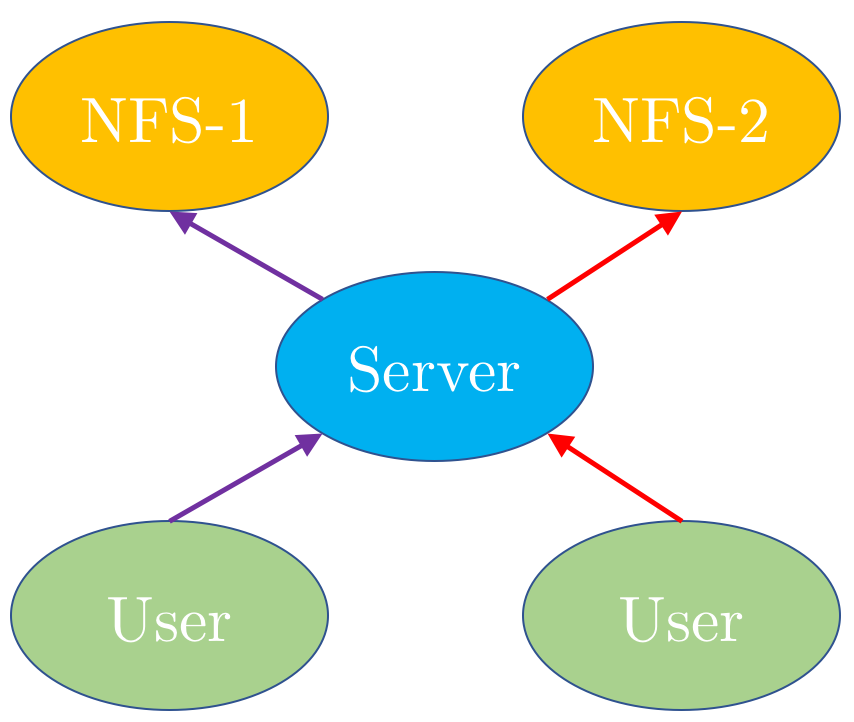
\includegraphics[height=0.2\textheight]{Fig1.png}
\caption{Structure of the workstation}
\end{figure}
\subsection{NFS Setup}
In NFS server, we must write the IP of the server in {\cs /etc/exports} to share directories to the workstation server.
It is important that the IP address of NFS server and workstation server must be constant.
In {\cs /etc/systemd/network/25-wired.network}, we add \\
\begin{minted}{shell}
[Match]
Name=enp0s8

[Network]
Address=192.168.100.3/24
\end{minted}
So that the IP addresses of NFS server and workstation server will be constant, which is the value given manually.
And the mount points are divided by grades of users. i.e. b03, b04, b05, etc. For example, in NFS-1, mount points are
{\cs /etc/nfsshare/\{b03902,b04902,b05902\}}
\subsection{Server Setup}
First, to decrease system loading, we use {\cs autofs} to mount the NFS directories. Only when the mounted points are used will they be mounted. 
If a mount point is not used for a given time, it will be unmounted. 

\section{Creating One Single User}
There are several steps we must follow to create a user:
   \begin{enumerate}
   \item Give a user name and password
   \item Set the home directory
   \item Link the home directory to NFS
   \item Change the owner of the home directory of the user.
   \end{enumerate}
Part of our script to do this is shown as following:
\begin{framed}
\begin{minted}{shell}
useradd $username -d /home/$grade/$username
echo -e "$username\n$username\n" | passwd $username >& /dev/null
mv /home/$grade/$username /autofs/$nfs/$grade/$username
ln -s /autofs/$nfs/$grade/$username /home/$grade/$username
chown -R $username /autofs/$nfs/$grade/$username
\end{minted}
\end{framed}
After execution of this script, we create a new user whose home directory is a symbolic link to the directory lies in NFS server.

\section{Creating or Deleting A Group of Users}
Suppose now we want to create accounts for freshmen, e.g. b06902\{001-120\}. 
Or more generally, we want to create or remove tens of or hundres of users.
The only data now we have is the current user\_list and the current distribution.
All we need to do is shown in Figure \ref{userChange}.
\begin{figure}[h]
\centering
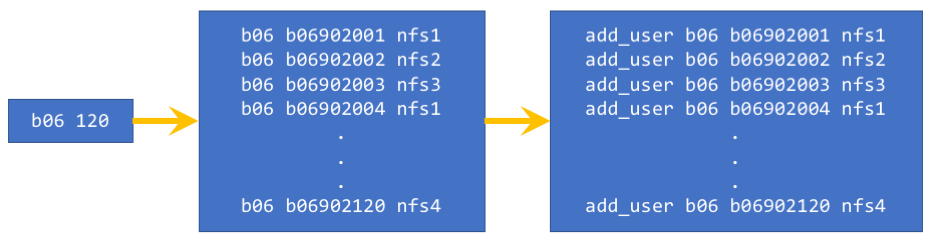
\includegraphics[width=\textwidth]{Fig2.png}
\caption{flow diagram of creating/removing a group of users}
\label{userChange}.
\end{figure}
There are two main changes we have to manage: on {\bf NFS server} side (distribution) and {\bf workstation server} side
(add/remove home directories). To be more clearly, following are steps we should do:
   \begin{enumerate}
   \item Backup the old user\_list and generate a new user\_list base on the old one upon need.
   \item Call {\cs distribute.out} and input the modified user\_list and old distribution.
   This program will compare those files to redistribute the newly created user or remove users to balance the distribution.
   \item Call {\cs group\_user\_change} to compare the previous user\_list and modified user\_list to figure out
   the home directories links we have to modify.
   \item Call {\cs update\_users.sh} and input distribution/changes and group\_user\_change to complete the modifications on workserver server and NFS server.
   \end{enumerate}

\section{Creating New NFS Server}
Steps are as following:
   \begin{enumerate}
   \item Setup NFS server for the workstation server to connect to and mount.
   \item Generate a new distribution list and find the users that are to be moved.
   \item Move the directories of these users to the new server.
   \item Update the symbolic links of the home directories of these users.
   \end{enumerate}
\subsection{Setup NFS Server}
For administrator's convinence, we can {\cs ssh} to the NFS server from workstation server and setup directories to share in
{\cs /etc/exports}. Then setup the autofs at the workstation side ({\cs /etc/auto.master, /etc/auto.nfs*})
\subsection{Find The Users To Be Moved}
We write a C++ program to do this job. The input is the previous distribution list, and output would be a new distribution list and
the modification we should make. We evenly take some users from each server, and move them to the new server.
\subsection{Move The Directories}
According to the modification, move the files of specified users from the previous nfs to the new nfs. This job is done using the same script as adding / deleting users since the input format is set the same.
\subsection{Update symbolic links}
In the end, we update the symbolic links of the home directories of these users according to the modification. After this, next time the users will login with new nfs servers keeping their home directories.
\section{Deleting Old NFS Server}
Quite similar to adding new NFS server, but now we need not to setup a new server.
Steps are as following:
   \begin{enumerate}
   \item Decide the new distribution.
   \item Move the directories to the new distributed NFS server.
   \item Update the symbolic link of the home directories of these users.
   \item Unmount the NFS servers and update the workstation server's autofs configuration.
   \end{enumerate}
\subsection{Decide The New Distribution}
Similar to adding new NFS server, we use a C++ program to distribute the users on the to-be-deleted server to other servers, and figure out the users that are influenced. We can delete multiple NFS servers at the same time to avoid moving the data more than once by deleting them one by one.
\subsection{Move The Directories to New NFS Server}
Same as the above. Use the same input format and script to do this job.
\subsection{Update Symbolic Link}
Same as the above.
\subsection{Unmount NFS servers}
In the end, the NFS servers we want to shutdown have no critical data now and can be safely removed from the system. Update the workstation server's autofs configuration and the NFS servers are off-duty.
\section{Difficulties}
Every single job looks easy, but how to integrate them for more convinient use is the main problem of this project.
Though each step looks easy, but we nead a clear structure to specify them. For example, I/O format should be 
accord between programs/scripts, and all programs and scripts should be packeted into a single script for administrator's convenience.

There are still some difficulties.

\subsection{Mount Points \& NFS Servers Arrangement}
In the ideal situation, the load of each mount point should be the same so that autofs can have the highest probability to unmount from time to time. Or in another scheme, we may put those who have the highest loadings in the same mount point so that other mount points can be unmounted longer. The loading of each NFS servers should be the same, and the amount of data should be fairly distributed so that when one of the servers fails, we need the least effort to restore the data and fix the system.

In reality, it's hard to determine the loading of each user in this project, so we assume each user has the same loading. Furthermore, with the requirement that we should change the least amount of user's data during adding/removing users/NFS servers, it's hard to come up with a good algorithm to maintain the optimal distribution when adding/removing users/NFS servers are all possible. Currently we use groups as mount points for simplicity (such as b05902, b06902, others), although number of users in each group may not be the same. Then we distribute the users into NFS servers with the same size. When adding/removing users/NFS servers, we maintain the same number of users in NFS servers so that the expected loading of each NFS server is the same and the effort to move the data is minimized.

\subsection{Selinux Context of home directories}
When we were trying to login into users we just created, we cannot set selinux context of the symbolic link correctly (seems to be unconfined\_u:object\_r:user\_home\_dir\_t:s0). The system will show ``permission denied'' when trying to load the home directory. However, the problem only occurs when trying to login with tty. But somehow  with ssh, this problem doesn't exist. We temporarily use selinux permissive to login with tty.

\section{Job Distribution}
\noindent
楊程皓: Structure discussion, Setup WS, NFS servers environment, Autofs configuration, User\_list, distribution structure \& algorithm, Scripts to refresh users/groups, Write the report. \\
\noindent
蔡承佑: Structure discussion, Symbolic link research, User privilege maintenance, Scripts to add/remove a single user, Randomness of distribution, Write the report. \\
\noindent
陳奕均: Structure discussion, Autofs research, Write the report, Presentation preparation. \\

\end{document}
